\chapter{Negative entropies}
\label{chapter_negative_entropies}

In the last chapters, we have found that parameters for which the entropy
becomes negative exist in the plane--plane as well as in the plane--sphere
geometry. In the plane--plane geometry negative entropies do not occur for
perfect reflectors and are thus caused by effects due to finite conductivity
and plasma oscillations of the metals. In contrast to this, negative entropies
are found in the plane--sphere geometry for perfect reflectors thus suggesting
a geometrical origin. In the large--distance limit we showed that the root of
the effect is due to a change of polarizations and the entropy is always
positive for temperatures higher than $T\approx1.5$. Throughout this chapter,
we will denote the temperature for fixed separation for which the entropy
changes its sign by $T_S(L/R)$. For smaller separations the effect becomes
less pronounced and our numerical results suggest that $T_S(L/R)$ tends to zero
for $L/R\to0$. This assumption is also strengthend by the PFA approximation. On
the one hand, the PFA yields positive values for the entropy for arbitrary
separations and temperatures. On the other hand, the approximation becomes
accurate for small separations. For these reasons, we expect negative entropies
to disappear for small separations. This argument can also be restated in terms
of geometry. For small separations the curvature of the sphere becomes small
and the geometry becomes similar to the plane--plane geometry. As the
curvature becomes small, changes of polarization may be neglected and the
effect of negative entropies vanishes.

\begin{figure}
    \begin{center}
    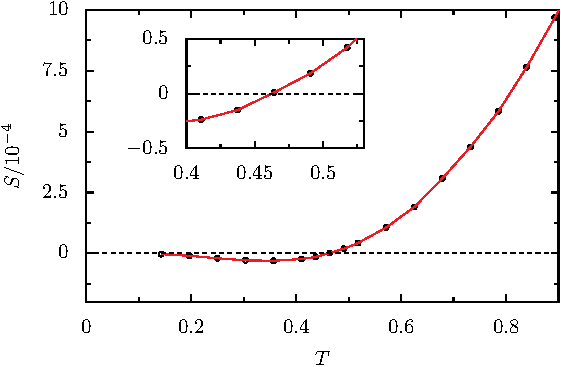
\includegraphics[scale=1]{plots/negentropies/S.pdf}
    \end{center}

    \caption{Entropy for $S$ for $L/R=0.02$ dependent on temperature. We find negative entropies for temperatures $T \lesssim 0.46$. ($\epsilon_p=10^{-8}$, $\lmax=300$)}

    \label{fig:neg_entropies_example}
\end{figure}

\begin{figure}[p]
  \begin{minipage}{\linewidth}
  \begin{center}
  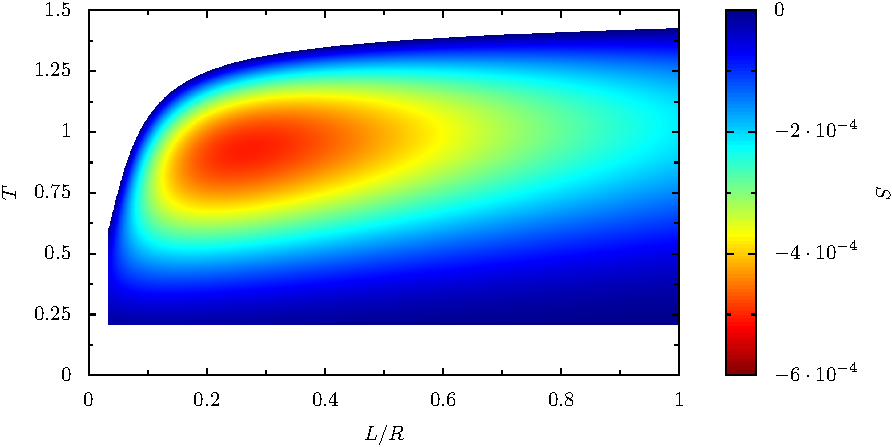
\includegraphics[scale=1]{plots/entropy_density_plot/plot_scaled.pdf}
  \subcaption{Negative entropy in scaled units for $0.207 \le T \le 1.5$.}
  \end{center}
  \end{minipage}
  \ \\ \ \\
  \begin{minipage}{\linewidth}
  \begin{center}
  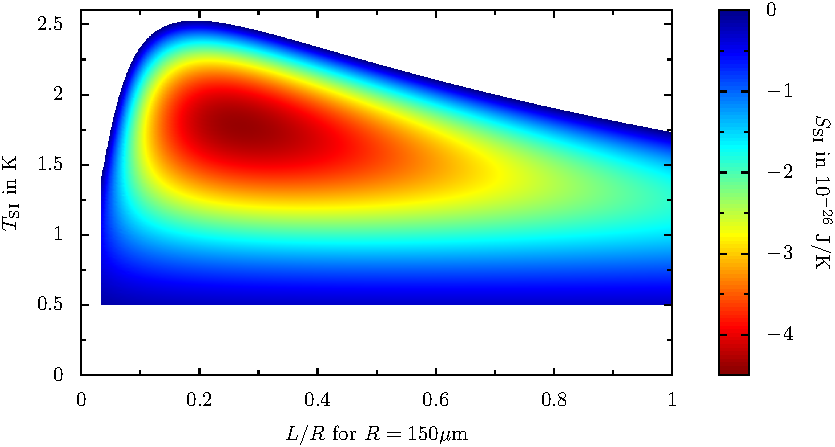
\includegraphics[scale=1]{plots/entropy_density_plot/plot_SI.pdf}
  \subcaption{Negative entropy in SI units for $R=150\mu\mathrm{m}$ and $0.5\mathrm{K} \le T_\SI \le 2.6\mathrm{K}$}
  \end{center}
  \end{minipage}

  \caption{Negative entropy dependent on temperature $T$ and separation $L/R$. The entropy
  is plotted a) in scaled units and b) in SI units for a sphere of radius $R=150\mu\mathrm{m}$ for
  separations $0.03415 \le L/R \le 1$ and temperatures according to subcaptions.
  White areas within this range correspond to positive values of the entropy.
  The minimum is located at $L/R=0.270$
  and a) $T=0.927$, and b) $T_\SI=1.77\mathrm{K}$.}

  \label{fig:neg_entropies_zoom}
\end{figure}

\begin{figure}
  \begin{minipage}{.5\linewidth}
  \begin{center}
  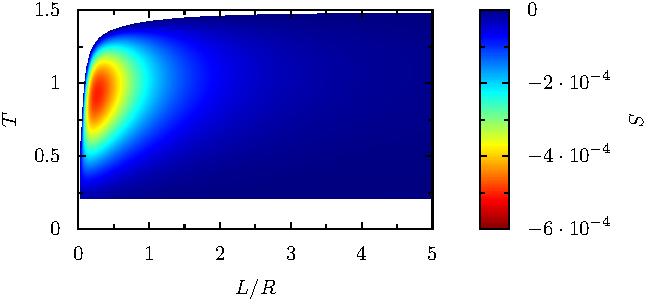
\includegraphics[scale=0.71]{plots/entropy_density_plot/plot_scaled_wide.pdf}
  \subcaption{scaled quantities}
  \end{center}
  \end{minipage}%
  \begin{minipage}{.5\linewidth}
  \begin{center}
  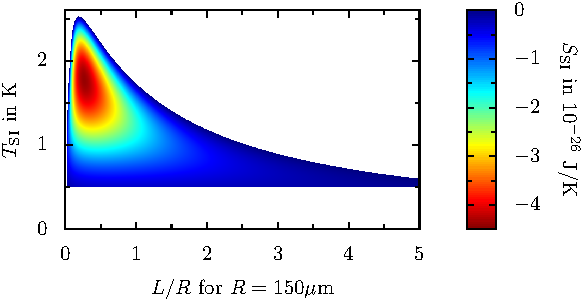
\includegraphics[scale=0.71]{plots/entropy_density_plot/plot_SI_wide.pdf}
  \subcaption{SI units for $R=150\mu\mathrm{m}$}
  \end{center}
  \end{minipage}

  \caption{Negative entropies for a) scaled quantities and b) in SI units for separations up to $L/R=5$.}

  \label{fig:neg_entropies}
\end{figure}

We now study the effect of negative entropies for arbitrary separations and
temperatures. In Fig. \ref{fig:neg_entropies_zoom} a) we plot the entropy
dependent on separation and temperature in the range $0.03415 \le L/R \le 1$
and $0.207 \le T \le 1.5$. White areas within this range correspond to positive
entropies. For large separations we rediscover the results of the
large--distance limit and the entropy is negative for temperatures lower than
$T < T_S(L/R) \approx 1.49$. Fig. \ref{fig:neg_entropies} a) shows the same
plot for separations up to $L/R=5$. For smaller separations $T_S(L/R)$
decreases, while the absolute values of the negative entropies increase down to
$L/R\approx0.3$. This may be understood as a result of two competing effects:
On the one hand, negative entropies are more distinct for large separations, or
small spheres respectively. In other words, the decrease of the ratio
$\mathcal{F}/\mathcal{F}(T=0)$ is stronger for large separations (cf. Fig.
\ref{fig:temp_intermediate}). On the other hand, the free energy decreases with
larger separations. Consequently, the effect of negative entropies increases
with separation, but at the same time the Casimir effect becomes less
pronounced. We find a minimum of the entropy for $L/R\approx0.270$ and
$T\approx0.927$. For smaller separations $T_S(L/R)$ continues to decrease. For
$L/R\approx0.034$ we find negative entropies for temperatures
$T_S\lesssim0.60$. Because of the arguments stated in the previous paragraph,
it seems plausible that $T_S(L/R)$ tends to zero for $L/R\to0$. This
assumption is also strengthened by Fig. \ref{fig:neg_entropies_example}. For
$L/R=0.02$ we find negative entropies for temperatures $T \lesssim 0.46$. The
numerical data for Fig. \ref{fig:neg_entropies_zoom} and Fig.
\ref{fig:neg_entropies} was obtained with identical parameters and resolution
as in section \ref{section_temp_intermediate}.

In Fig. \ref{fig:neg_entropies_zoom} we plot the negative entropy in SI units
for a sphere of radius $R=150\mu\mathrm{m}$ which is a typical size in experiments \cite{2012IJMPA2760013L}.
We want to remind the reader that
quantities measured in SI units are labeled with a subscript ``SI''.
While the separation
$L/R$ remains constant when changing to SI units, the temperature of the
minimum of the entropy is now located at $T_\SI = 1.77\mathrm{K}$. The minimum in
SI units for arbitrary values of $R$ is given by
\eqref{eq:scattering_ps_scaled}
\begin{equation}
T_\SI \approx \frac{\hbar \c}{2\pi \, \kb \, R(1+L/R)} \, T = \frac{0.927}{1.270} \, \frac{\hbar \c}{2\pi \, \kb \, R}.
\end{equation}
For smaller spheres this temperature increases and corresponds to ambient
temperature for $R\approx1.2\mu\mathrm{m}$. While $T_S(L/R)$
tends to a constant value for large separations in scaled
units, $T_S(L/R)$ tends to zero for SI units. This is caused by the
scaling \eqref{eq:scattering_ps_scaled}. In SI units the entropy is given by
\begin{equation}
S_\SI = - \frac{\partial \mathcal{F}_\SI}{\partial T_\SI} = -\frac{\hbar\c}{\mathcal{L}} \frac{\partial\mathcal{F}}{\partial T} \frac{\partial T}{\partial T_\SI}
= 2\pi \kb S(T) = 2\pi \kb S\left(T = \frac{2\pi\kb R (1+L/R)}{\hbar\c}T_\SI\right).
\end{equation}
For large separations the entropy $S$ is negative for $T\lesssim1.5$. From this
it follows that $T_S(L/R)$ decreases for large separations like
\begin{equation}
T = \frac{2\pi \kb R (1+L/R)}{\hbar\c} T_\SI \lesssim 1.5 \\
\Leftrightarrow \\
T_\SI \lesssim 1.5 \frac{\hbar\c}{2\pi \kb R (1+L/R)} \propto \frac{1}{1+L/R}.
\end{equation}
This can be seen in Fig. \ref{fig:neg_entropies} b) for separations up to $L/R=5$.

We now address the question about the relevance of negative entropies in the
Casimir effect. We have found non-monotonic behaviour of the free energy over
a wider range of parameters. However, the definition of the entropy from
statistical mechanics claims that the entropy is positive. This contradiction
is resolved by the fact that the Casimir free energy is an interaction energy.
We are actually only considering a subsystem of the full system
\cite{1367-2630-8-10-236}. For this reason, the Casimir entropy corresponds to
a difference of two entropies. There is no physical reason why the difference
of two entropies ought to be positive \cite{2009PhRvE80d1113I,
2010IJMPA25.2313P}.
